\documentclass[12pt]{report}
\usepackage[paper=letterpaper,margin=3cm]{geometry}
\usepackage{amsmath}
\usepackage{amssymb}
\usepackage{amsfonts}
\usepackage{newtxtext, newtxmath}
\usepackage{enumitem}
\usepackage{titling}
\usepackage{nccmath}
\usepackage[colorlinks=true]{hyperref}
\usepackage[utf8]{inputenc}
\usepackage{graphicx}
\usepackage{tcolorbox}
\usepackage{pgfplots}
\graphicspath{ {images/} }
\tcbuselibrary{raster}

% Externalising the figures used:
\usepgfplotslibrary{external}
\tikzexternalize

\setlength{\droptitle}{-6em}
\pgfplotsset{width=10cm,compat=1.18}
% Enter the specific assignment number and topic of that assignment below, and replace "Your Name" with your actual name.
\title{Assignment \# 4: MATH1051} 
\author{Jamie Chen\\ \text{Student Number:} \texttt{48093189} \\ \text{Semester 2, 2023}}
\date{\today}

\begin{document}
\maketitle
\begin{enumerate}[leftmargin=\labelsep]
%% Question 1

    \item {\bf (1 mark each)} Determine the domains (as a subset of $\mathbb{R}$) of the functions:
        \begin{enumerate}
            \item $f_1(x)=\frac{1}{e^x-e^{-x}}$
                \begin{itemize}[label={}]
                    \item 
                    \item The domain of this function $f_1(x)$ is $\mathbb{R} \setminus \{0\}$.
                    \item 
                \end{itemize}
            \item $f_2(x)=\frac{1}{\sqrt{4-x^2}}$
                \begin{itemize}[label={}]
                    \item
                    \item The domain of this function $f_2(x)$ is $(-2,2)$ (non-inclusive).
                    \item 
                \end{itemize}
            \item $f_3(x)= \log \arccos x$ 
                \begin{itemize}[label={}]
                    \item
                    \item The domain of this function $f_3(x)$ is $[-1,1]$ (inclusive). 
                    \item 
                \end{itemize}
        \end{enumerate}
            
%% New Page
\newpage
%% Question 2  

    \item {\bf (3 marks)} Given is the function $g(x)=x^2+3x$. For a second function $f$ with $f(3)=0$ we find $(g \circ f)(x)=x^2-3x$. What is the function $f$? Is $f$ unique?
        \begin{itemize}[label={}]
            \item The function $f$ can be a simple linear function, such as $f(x)=x-3$. 
            \begin{equation*}
                \begin{split}
                    (g \circ f)(x) &= g(f(x)) \\
                    &= (x-3)^2+3(x-3) \\
                    &= x^2-6x+9+3x-9 \\
                    &= x^2-3x
                \end{split}
            \end{equation*}
            However, there are other functions that can be used to achieve the same result. (NOT PROVEN YET)
            %TODO Prove that there are other functions that can be used to achieve the same result.
            
        \end{itemize}

%% New Page
\newpage        
%% Question 3
    
    \item {\bf (1 mark each)} Determine which of the following functions are 1-1? Prove your answer.
        \begin{enumerate}
            \item $f_1(x)=e^{-x^2}$
                \begin{tcolorbox}
                    \begin{itemize}[label={}]
                        \item Defined in the workbook:
                        \begin{quote}
                            A function $f: X\to Y$ is called {\bf one-to-one} (or {\bf injective}) if $\forall x_1,x_2 \in \mathbb{R} \cap X$, $f(x_1)=f(x_2)$ $\implies$ $x_1=x_2$.
                        \end{quote}
                        \item
                        \item The function $f_1(x)=e^{-x^2}$ is one-to-one as it is a strictly decreasing function. Additionally, if we follow the definition of a one-to-one function:
                        \begin{equation*}
                            \begin{split}
                                f_1(x_1) &= f_1(x_2) \\
                                e^{-x_1^2} &= e^{-x_2^2} \\
                                \ln (e^{-x_1^2}) &= \ln (e^{-x_2^2}) \\
                                -x_1^2 &= -x_2^2 \\
                                x_1^2 &= x_2^2 \\
                                \implies x_1 &= x_2
                            \end{split}
                        \end{equation*}
                        \item Therefore, the function $f_1(x)=e^{-x^2}$ is one-to-one.
                        \item You can see that there are other things:
                    \end{itemize}
                \end{tcolorbox}
                %TODO Add a graph of the function $f_1(x)=e^{-x^2}$.
\newpage
            \item $f_2(x)=2x^2-3x+1$
                \begin{tcolorbox}
                    \begin{itemize}[label={}]
                        \item The function $f_2(x)=2x^2-3x+1$ is not one-to-one. There are several reasons for this:
                        \begin{enumerate}
                            \item[1.] The function $f_2(x)$ is not strictly increasing or decreasing.
                            \item[2.] The function $f_2(x)$ is a quadratic function, and therefore can have two values of $x$ that correspond to the same value of $y$. 
                            \item[3.] Using the definition of a one-to-one function:
                            \begin{equation*}
                                f_1(x_1) = f_1(x_2) \implies x_1 = x_2 \\
                            \end{equation*} 
                            \begin{equation*}
                                2x_1^2-3x_1+1 = 2x_2^2-3x_2+1 \implies x_1 = x_2
                            \end{equation*}
                            \item[] We can see that the function $f_2(x)$ is not one-to-one as there are multiple values of $x$ that correspond to the same value of $y$.
                            \begin{center}
                                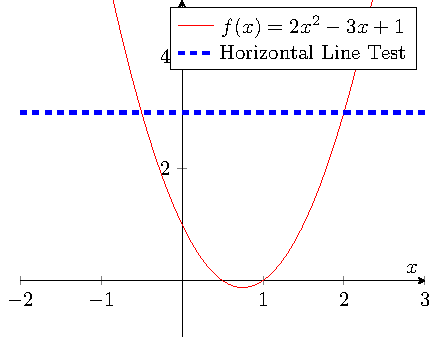
\includegraphics[width=0.8\linewidth]{lib/figures/Figure1.pdf}
                            \end{center}
                        \end{enumerate}
                    \end{itemize}
                \end{tcolorbox}

\newpage
            \item $f_3(x)=|x|+2 \cdot x$
                \begin{tcolorbox}
                    \begin{itemize}[label={}]
                        \item The function $f_3(x)=|x|+2 \cdot x$ is one-to-one. There are several reasons for this (using the definition of a one-to-one function):
                        \begin{equation*}
                            \begin{array}{r@{~=~}l}
                                f_3(x_1) & f_3(x_2) \\ [2ex]
                                |x_1|+2 \cdot x_1 & |x_2|+2 \cdot x_2 \\ [2ex]
                            \end{array}
                        \end{equation*}
                        \item In this case, lets consider that there are two cases:
                        \item The first case is when $x_1,x_2 \geq 0$:
                        \item In this case, we can assume that $|x_1|=x_1$ and $|x_2|=x_2$. We can then determine the equation for this case:
                        \begin{equation*}
                            |x_1|+2 \cdot x_1 = |x_2|+2 \cdot x_2
                        \end{equation*}
                        \item Simplifying this equation gives us:
                        \begin{equation*}
                            3x_1 = 3x_2
                        \end{equation*}
                        \item Dividing both sides by 3 gives us:
                        \begin{equation*}
                            x_1 = x_2
                        \end{equation*}
                        \item We can now determine the second case.
                        \item The second case is when $x_1,x_2 < 0$:
                        \item In this case, we can assume that $|x_1|=-x_1$ and $|x_2|=-x_2$. We can then determine the equation for this case:
                        \begin{equation*}
                            -x_1+2 \cdot x_1 = -x_2+2 \cdot x_2
                        \end{equation*}
                        \item Simplifying this equation gives us:
                        \begin{equation*}
                            x_1 = x_2
                        \end{equation*}
                        \item After determining both cases for the absolute value function, we can see that the function $f_3(x)=|x|+2 \cdot x$ is one-to-one.
                    \end{itemize}
                \end{tcolorbox}
        \end{enumerate}
            
%% New Page
\newpage
%% Question 4 

    \item {\bf (1 mark each)} Determine what the following limits are or show that they do not exist.
        \begin{enumerate}
            \item $ {\lim \limits_{{n\rightarrow \infty}}} \frac{(n^2+4 n-27)(n^3-1)}{(n(n-1))^2} $
                \begin{tcolorbox}
                    \begin{equation*}
                        \begin{array}{r@{~=~}l}
                            {\lim \limits_{{n\rightarrow \infty}}} \frac{(n^2+4 n-27)(n^3-1)}{(n(n-1))^2} & {\lim \limits_{{n\rightarrow \infty}}} \frac{n^5+4n^4-27n^3-n^3+1}{n^4-2n^3+n^2} \\ [2ex]
                            & {\lim \limits_{{n\rightarrow \infty}}} \frac{n^5+4n^4-28n^3+1}{n^4-2n^3+n^2} \\ [2ex]
                            & {\lim \limits_{{n\rightarrow \infty}}} \frac{n+4-\frac{28}{n}+\frac{1}{n^3}}{1-\frac{2}{n}+\frac{1}{n^2}} \\ [2ex]
                            & \frac{\infty}{1} \\ [2ex]
                            & \infty
                        \end{array}
                    \end{equation*}
                \end{tcolorbox}
            \item $\lim \limits_{n\rightarrow \infty} \frac{3n^2-9n + 48}{4n^3}$
                \begin{tcolorbox}
                    \begin{equation*}
                        \begin{array}{r@{~=~}l}
                            {\lim \limits_{{n\rightarrow \infty}}} \frac{3n^2-9n + 48}{4n^3} & {\lim \limits_{{n\rightarrow \infty}}} \frac{3-\frac{9}{n} + \frac{48}{n^2}}{4n} \\ [2ex]
                            & {\lim \limits_{{n\rightarrow \infty}}} \frac{3}{4n} - \frac{9}{4n^2} + \frac{12}{n^3} \\ [2ex]
                            & 0 \quad \text{Since the limit of } \frac{1}{n} = 0 \text{ as } n \rightarrow \infty.
                        \end{array}
                    \end{equation*}
                \end{tcolorbox}
            \item $\lim \limits_{n\rightarrow \infty} \frac{(3n+1)^3-27n^3}{n^2}$
                \begin{tcolorbox}
                    \begin{equation*}
                        \begin{array}{r@{~=~}l}
                            {\lim \limits_{{n\rightarrow \infty}}} \frac{(3n+1)^3-27n^3}{n^2} & {\lim \limits_{{n\rightarrow \infty}}} \frac{27n^3+27n^2+9n+1-27n^3}{n^2} \\ [2ex]
                            & {\lim \limits_{{n\rightarrow \infty}}} \frac{27n^2+9n+1}{n^2} \\ [2ex]
                            & {\lim \limits_{{n\rightarrow \infty}}} (27+\frac{9}{n}+\frac{1}{n^2}) \\ [2ex]
                            & 27
                        \end{array}
                    \end{equation*}
                    \begin{itemize}[label={}]
                        \item $\therefore$ The limit is 27 as $n \rightarrow \infty$.
                    \end{itemize}
                \end{tcolorbox}
\newpage
            \item $\lim \limits_{n\rightarrow \infty} \frac{2n^2}{2n-1}-n$
                \begin{tcolorbox}
                    \begin{equation*}
                        \begin{array}{r@{~=~}l}
                            {\lim \limits_{{n\rightarrow \infty}}} \frac{2n^2}{2n-1}-n & {\lim \limits_{{n\rightarrow \infty}}} \frac{2n^2}{2n-1}-\frac{n(2n-1)}{2n-1} \\ [2ex]
                            & {\lim \limits_{{n\rightarrow \infty}}} \frac{2n^2-n(2n-1)}{2n-1} \\ [2ex]
                            & {\lim \limits_{{n\rightarrow \infty}}} \frac{2n^2-2n^2+n}{2n-1} \\ [2ex]
                            & {\lim \limits_{{n\rightarrow \infty}}} \frac{n}{2n-1} \\ [2ex]
                            & {\lim \limits_{{n\rightarrow \infty}}} \frac{1}{2-\frac{1}{n}} \\ [2ex]
                            & \mfrac{1}{2} \quad \text{Since the limit of } \frac{1}{n} = 0 \text{ as } n \rightarrow \infty.
                        \end{array}
                    \end{equation*}
                    \begin{itemize}[label={}]
                        \item Therefore, the limit is $\frac{1}{2}$ as $n \rightarrow \infty$.
                    \end{itemize}
                \end{tcolorbox}
            \item $\lim \limits_{n\rightarrow \infty} \sqrt{n(n+1)}-n$
                \begin{tcolorbox}
                    \begin{itemize}[label={}]
                        \item In this limit, we can find the limit by rationalising the numerator.
                        \item To do this we can multiply the numerator and denominator by the conjugate of the numerator:
                        \begin{equation*}
                            \begin{array}{r@{~=~}l}
                                {\lim \limits_{{n\rightarrow \infty}}} \sqrt{n(n+1)}-n & {\lim \limits_{{n\rightarrow \infty}}} \sqrt{n(n+1)}-n \times \frac{\sqrt{n(n+1)}+n}{\sqrt{n(n+1)}+n} \\ [2ex]
                                & {\lim \limits_{{n\rightarrow \infty}}} \frac{n(n+1)-n^2}{\sqrt{n(n+1)}+n} \\ [2ex]
                            \end{array}
                        \end{equation*}
                        \item We can then simplify the equation to find the limit:
                        \begin{equation*}
                            \begin{array}{r@{~=~}l}
                                & {\lim \limits_{{n\rightarrow \infty}}} \frac{n^2+n-n^2}{\sqrt{n(n+1)}+n} \\ [2ex]
                                & {\lim \limits_{{n\rightarrow \infty}}} \frac{n}{\sqrt{n(n+1)}+n} \\ [2ex]
                                & {\lim \limits_{{n\rightarrow \infty}}} \frac{1}{\sqrt{1+\frac{1}{n}}+1} \\ [2ex]
                                & \frac{1}{2} \quad \text{Since the limit of } \frac{1}{n} = 0 \text{ as } n \rightarrow \infty.
                            \end{array}
                        \end{equation*}
                    \end{itemize}
                \end{tcolorbox}
        \end{enumerate}

%% New Page
\newpage
%% Question 5

    \item {\bf (1 mark each)} Consider the sequence $a_n$ defined by the recursion
        \begin{equation}
            a_n=a_{n-1}-\frac{1}{4}a_{n-2}
        \end{equation} for $n=3,4,5,\dots$.
        \begin{enumerate}
            \item Calculate $h$ such that $a_n=h^{n-1}$ fulfils the recursive definition.
                \begin{tcolorbox}
                    \begin{itemize}[label={}]
                        \item To calculate $h$ we can substitute $a_n=h^{n-1}$ into the recursive definition:
                        \begin{equation*}
                            h^{n-1}=h^{n-2}-\frac{1}{4}h^{n-3}
                        \end{equation*}
                        \item We can now divide both sides by $h^{n-3}$:
                        \begin{equation*}
                            h^2=h- \frac{1}{4}
                        \end{equation*}
                        \item Solving h in terms of the quadratic formula:
                        \begin{equation*}
                            h=\frac{-(-1) \pm \sqrt{1-4 \cdot 1 \cdot \frac{1}{4}}}{2 \cdot 1}
                        \end{equation*}
                        \begin{equation*}
                            h=\frac{1 \pm \sqrt{1-1}}{2}
                        \end{equation*}
                        \begin{equation*}
                            h=\frac{1 \pm 0}{2}
                        \end{equation*}
                        \begin{equation*}
                            \therefore h=\frac{1}{2}
                        \end{equation*}
                    \end{itemize}
                \end{tcolorbox}
            \item What is the limit of the sequence $a_n$ (if it exists)?
                \begin{tcolorbox}
                    \begin{itemize}[label={}]
                        \item To find the limit of the sequence $a_n$ we can use the formula.
                    \end{itemize}
                \end{tcolorbox}
        \end{enumerate}

%% New Page
\newpage
%% Question 6

    \item {\bf (1 mark each)} Given is the sequence $b_n$ defined in recursive form
        \begin{equation*}
            b_n=\frac{1}{2}\left(b_{n-1}+\frac{A}{b_{n-1}} \right)
        \end{equation*} for a given $A>0$. You can assume that all values of $b_n$ are non-zero.
        \begin{enumerate}
            \item Use your calculator (or MATLAB) to calculate the first four values of the sequence $b_n$ starting from $b_1=A$ (this is for $n=1,2,3,4$). Inspecting these values do you expect the sequence to be convergent or to be divergent?
                \begin{itemize}[label={}]
                    \item 
                \end{itemize}
            \item Assume you know the sequence $b_n$ is converging, what would be its limit (or its limits)? Justify your answer. Is it consistent with your result of part (a)?
                \begin{itemize}[label={}]
                    \item 
                \end{itemize}
        \end{enumerate}

%% New Page
\newpage
%% Question 7

    \item {\bf (1 mark each)} Assume you have given a sequence $c_n$ with non-zero values ($c_n\neq0$ for $n=1,2,\dots$) that fulfils the condition
        \begin{equation}
            \left|\frac{c_n}{c_n-1}\right|\leq q
        \end{equation} for all $n=1,2,3,\dots$ for some fixed constant q with $0<q<1$.
        \begin{enumerate}
            \item Show that $c_n\to0$ for $n\to \infty$. (Hint: use the squeeze theorem)
                \begin{itemize}[label={}]
                    \item 
                \end{itemize}
            \item Use the result from part(a) to show that $\displaystyle{\lim_{n \to \infty}}\,\,\, \frac{2^n}{n!}=0$.
                \begin{itemize}[label={}]
                    \item 
                \end{itemize}
            \item Again: use the result from part(a) to show that $\displaystyle{\lim_{n \to \infty}}\,\,\, \frac{1}{3^nn^3}=0$.
        \end{enumerate}


\end{enumerate}
\end{document}